% 1977 年天津卷第 4(1) 题：河对岸建筑物高度测量
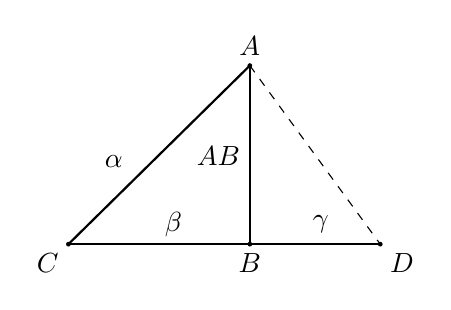
\begin{tikzpicture}[scale=0.72,>=stealth]
  \coordinate (B) at (0.7,0.1);
  \coordinate (A) at (0.7,3.25);
  \coordinate (C) at (-2.5,0.1);
  \coordinate (D) at (3.0,0.1);
  \draw[thick] (A)--(B);
  \draw[thick] (C)--(D);
  \draw[thick] (C)--(A);
  \draw[thick] (C)--(B);
  \draw[thick] (D)--(B);
  \draw[dashed] (A)--(D);
  \fill (A) circle (1.2pt) node[above] {$A$};
  \fill (B) circle (1.2pt) node[below] {$B$};
  \fill (C) circle (1.2pt) node[below left] {$C$};
  \fill (D) circle (1.2pt) node[below right] {$D$};
  \node at (-1.7,1.55) {$\alpha$};
  \node at (-0.65,0.45) {$\beta$};
  \node at (1.95,0.45) {$\gamma$};
  \node[left] at (0.7,1.65) {$AB$};
\end{tikzpicture}
